\documentclass{article}
\usepackage[UTF8]{ctex}
\usepackage{pythonhighlight}
\usepackage{markdown}
\usepackage{listings}
\lstset{
    basicstyle          =   \tt,          % 基本代码风格
    identifierstyle=\color{brown!80!black},
    keywordstyle        =   \color{purple}\bfseries,          % 关键字风格
    commentstyle        =   \rmfamily\itshape,  % 注释的风格,斜体
    stringstyle         =   \ttfamily,  % 字符串风格
    flexiblecolumns,                % 别问为什么,加上这个
    numbers             =   left,   % 行号的位置在左边
    showspaces          =   false,  % 是否显示空格,显示了有点乱,所以不现实了
    numberstyle         =   \zihao{-5}\ttfamily,    % 行号的样式,小五号,tt等宽字体
    showstringspaces    =   false,
    captionpos          =   t,      % 这段代码的名字所呈现的位置,t指的是top上面
    frame               =   lrtb,   % 显示边框
    backgroundcolor=\color[RGB]{245,245,244},
}


% Language setting
% Replace `english' with e.g. `spanish' to change the document language
\usepackage[english]{babel}
\usepackage{float}
% Set page size and margins
% Replace `letterpaper' with `a4paper' for UK/EU standard size
\usepackage[letterpaper,top=2cm,bottom=2cm,left=3cm,right=3cm,marginparwidth=1.75cm]{geometry}

% Useful packages
\usepackage{amsmath}
\usepackage{graphicx}
\usepackage[colorlinks=true, allcolors=blue]{hyperref}

\title{数逻实验报告Lab10}
\author{雷远航}

\begin{document}

\maketitle

\begin{abstract}
    同步时序电路设计
\end{abstract}

\section*{一、操作方法与实验步骤}

\subsection*{任务1: 4位同步二进制计数器}

\subsubsection*{原理图实现:}
以原理图方式对4位同步二进制计数器进行实现,原理图如下
\begin{figure}[H]
    \centering
    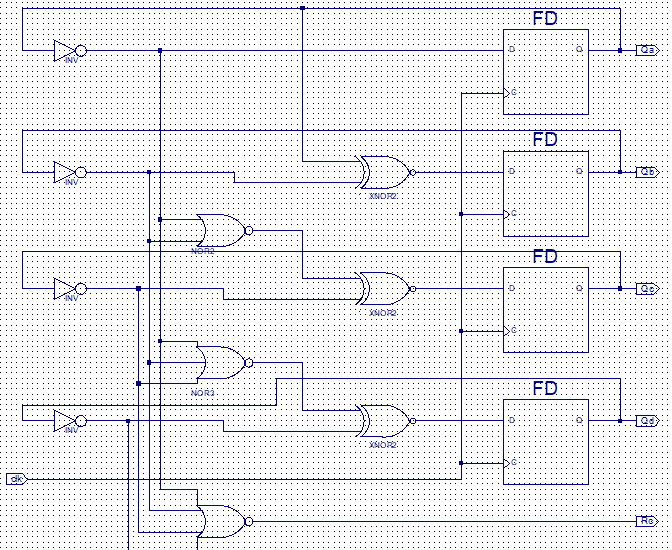
\includegraphics[width=0.7\textwidth]{lab10p/14.png}
    \caption{\label{Lab10}下板照片}
    \end{figure}

\subsubsection*{测试文件内容:}

通过以下的testbench代码进行测试并得到对应的测试波形.
\begin{lstlisting}[language=verilog]
    `timescale 1ps/1ps


module Counter4b_tb();
  
  reg clk;
  wire Qa;
  wire  Qb; 
  wire  Qc;
  wire Qd;
  wire Rc;
  Counter4b u0 (.clk(clk),.Qa(Qa),.Qb(Qb),.Qc(Qc),.Qd(Qd),.Rc(Rc));
  
  initial begin
    
    repeat(50) begin
      clk = 0; #10;
      clk = 1; #10;
    end
   
  end

endmodule 
\end{lstlisting}

\subsection*{任务2: 16位可逆二进制同步计数器(完成Bonus)}

使用Verilog实现16位可逆二进制同步计数器,并且增加了RESET信号,实现将计数器
信号重置为0.
\subsubsection*{Verilog实现(完成Bonus):}

\begin{lstlisting}[language=verilog]
    module RevCounter( 
        input wire clk,
        input wire s,
        input wire rst,
        output reg [15:0] cnt=0,
        output wire Rc
    );
         
        
    initial begin
        cnt = 0;
    end
    
    assign Rc = (~s & (~|cnt) | (s & (&cnt)));
    
    always @(posedge clk) begin
        if(rst==1'b1) begin
            cnt <= 0;
        end
        if(rst==1'b0) begin
        if(s==1'b1) begin
            cnt <= cnt + 1;
        end
        else begin
            cnt <= cnt - 1; 
        end
        end
    
    end
    
    endmodule
    

\end{lstlisting}


\subsubsection*{测试文件:}
通过以下的testbench代码对上述的Verilog实现可逆计数器进行测试,并且生成对应的测试波形

\begin{lstlisting}[language=verilog]
    `timescale 1ps/1ps
    `include "RevCounter.v"
    
    module RevCounter_tb ();
    
    reg clk;
    reg s;
    wire Rc;
    wire [15:0] cnt;
    
    RevCounter u0 (.clk(clk),.s(s),.cnt(cnt),.Rc(Rc));
    
    initial begin
        $dumpfile("RevCounter.vcd");
        $dumpvars(1, RevCounter_tb);
    
        s = 1;
    
        repeat (6) begin
            clk = 0; #10;
            clk = 1; #10;
        end
    
        s = 0;
    
        repeat (10) begin
            clk = 0; #10;
            clk = 1; #10;
        end
    
        s = 1;
    
        repeat (5) begin
            clk = 0; #10;
            clk = 1; #10;
        end
    
    
    end
    
    
    endmodule
\end{lstlisting}

\section*{二、实验结果与分析}

\subsection*{四位同步二进制计数器的测试波形与解释:}

    \begin{figure}[H]
    \centering
    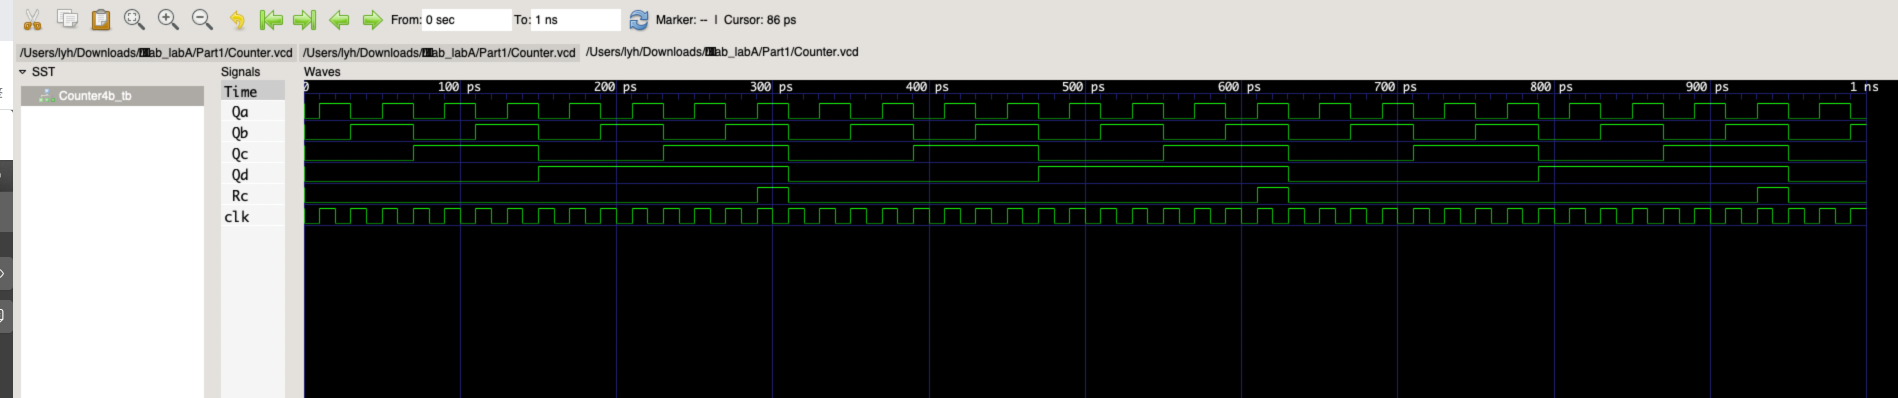
\includegraphics[width=1\textwidth]{lab10p/2.png}
    \caption{\label{Lab10}波形图}
    \end{figure}

原理图中利用了时序逻辑实现了四位同步计数器,{Qd,Qc,Qb,Qa}四位表示该数字,在每个正边沿的时钟信号时刻,
输出的信号会根据设计的逻辑进行更新,输出的结果波形图最终显示为,在每个时钟周期依次显示出递增的数字,当
数字为4'b1111时,Rc信号为1,将输出的信号全部置0.

\subsection*{十六位可逆二进制计数器的测试波形与解释:}
\begin{figure}[H]
    \centering
    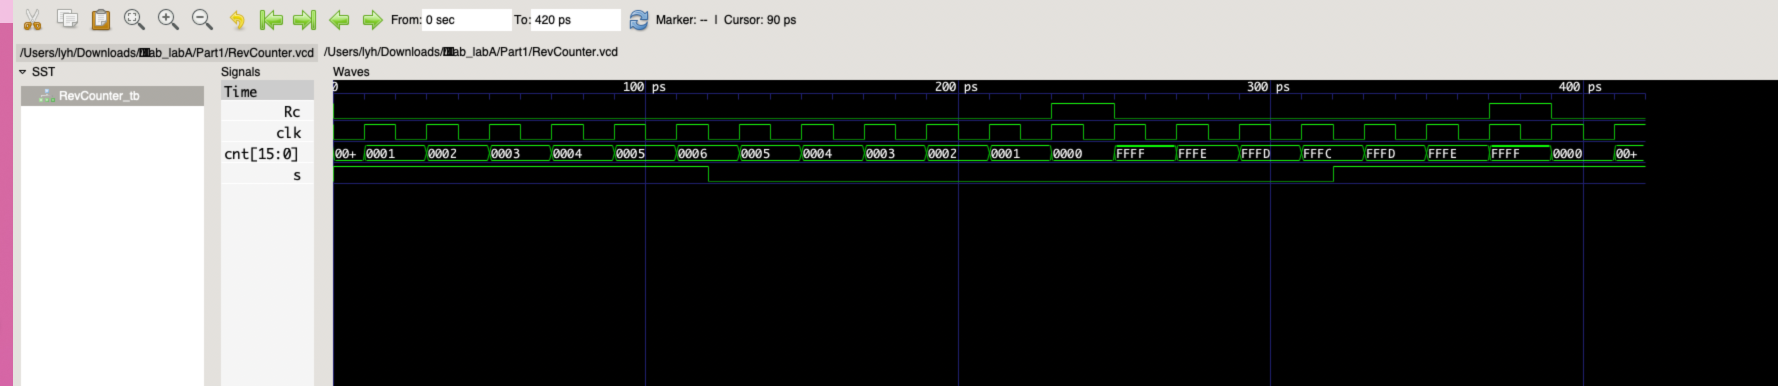
\includegraphics[width=1\textwidth]{lab10p/1.png}
    \caption{\label{Lab10}波形图}
    \end{figure}

当s信号为1时,表示当前处于递增的状态,在每个时钟正边沿的时刻,对应的输出数字会增加1,
如:在波形图中从4'h0000增加到4'h0006.

当s信号为0时,表示当前处于递减状态,在每个时钟正边沿的时刻,对应的输出数字会减1,
如:在波形图中从4'h0006到4'h0000.

在处于递减状态时,输出的数字为4'h0000时Rc信号为1,下一个时钟周期输出4'hFFFF.在处于递增状态时,输出的数字为
4'hFFFF时,Rc信号为1,下一个时钟周期输出4'h0000.

在波形图中可以看出在Rc=1,的两个时刻输出的数字符合以上的情况.

\subsection*{两个工程的下板照片与对应的文字解释:}

\subsubsection*{4位同步二进制计数器:}
    \begin{figure}[H]
    \centering
    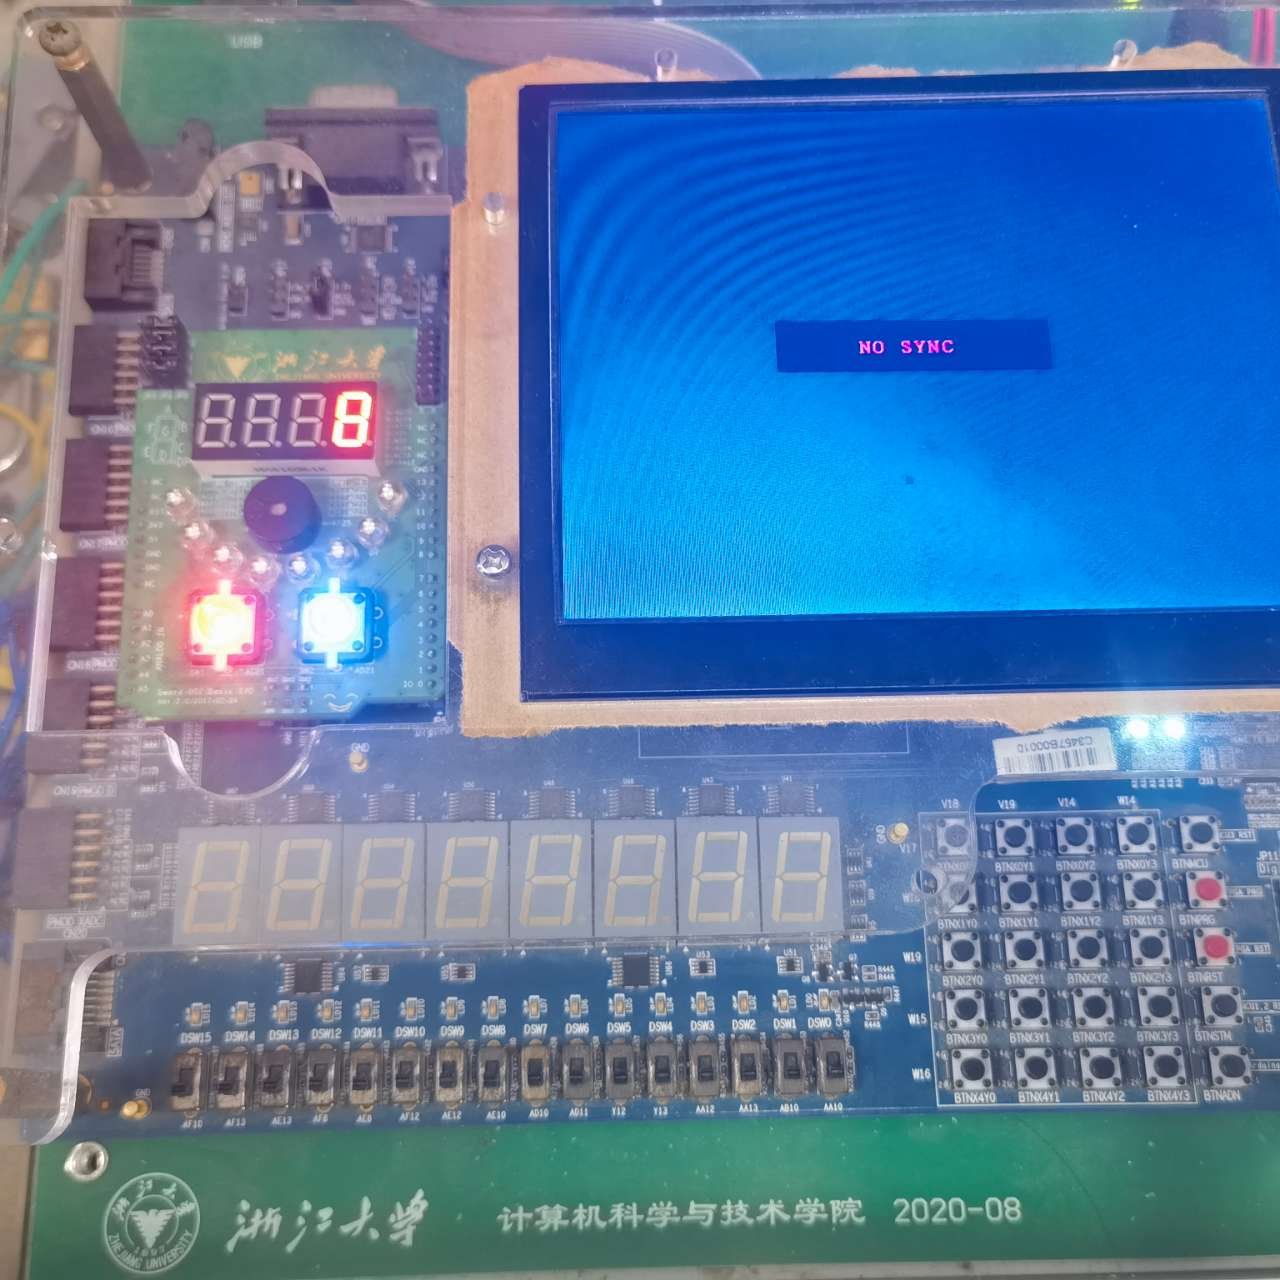
\includegraphics[width=0.5\textwidth]{lab10p/3.jpg}
    \caption{\label{Lab10}下板照片}
    \end{figure}

    \begin{figure}[H]
    \centering
    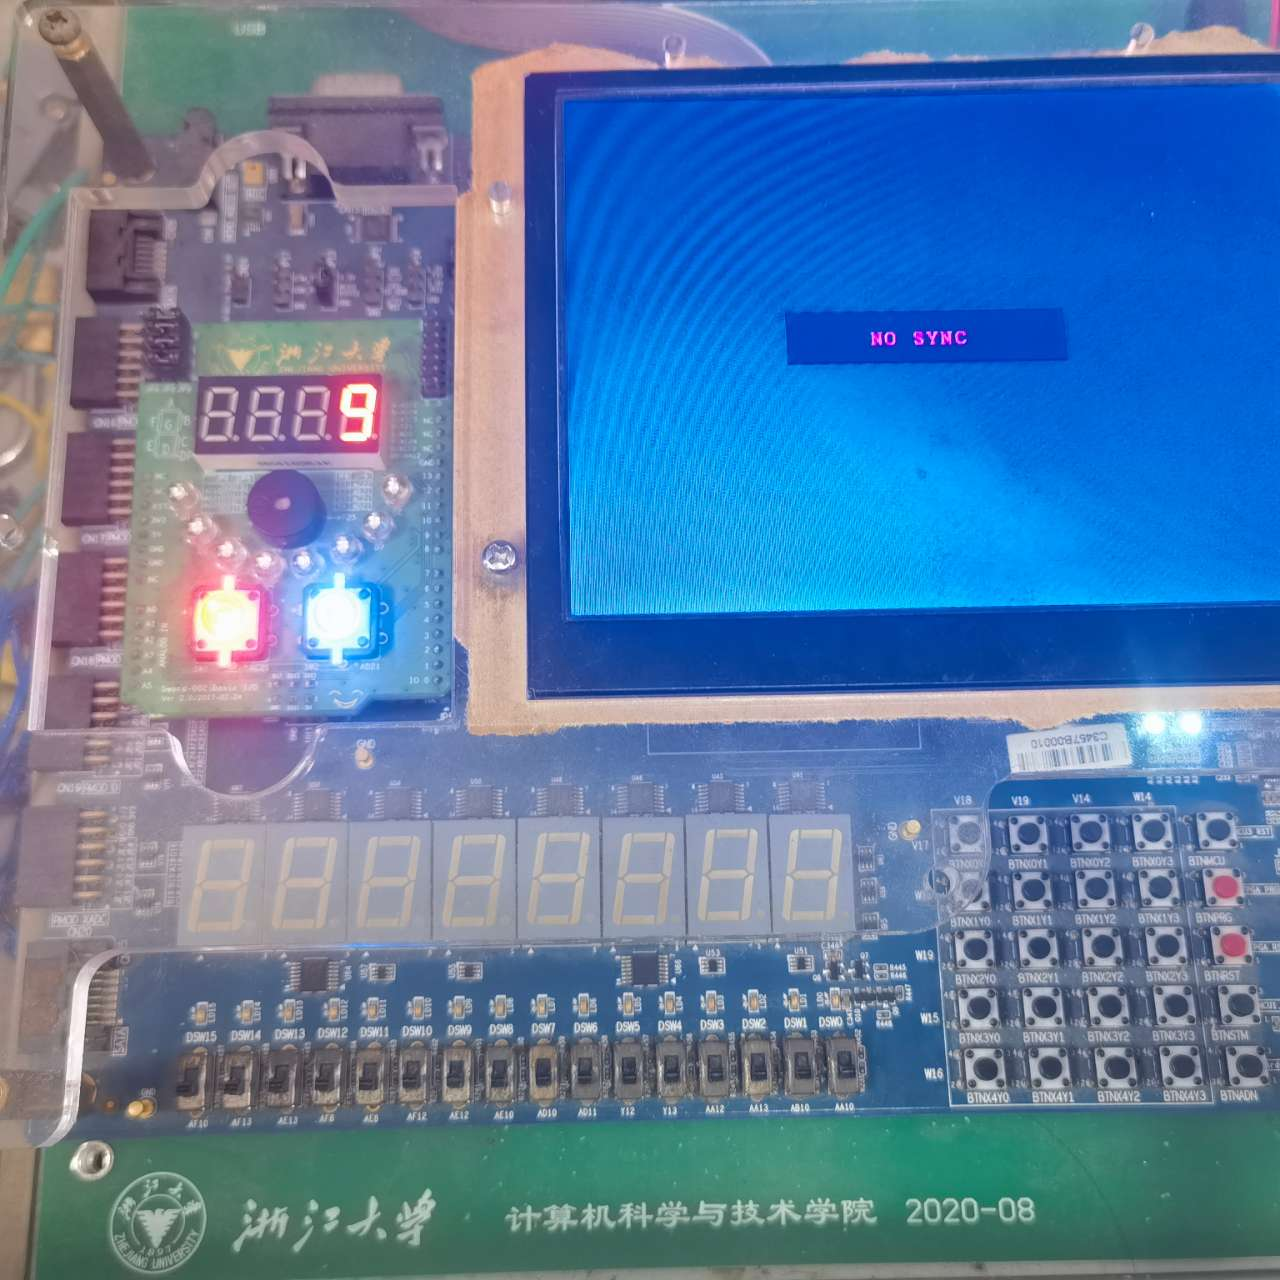
\includegraphics[width=0.5\textwidth]{lab10p/4.jpg}
    \caption{\label{Lab10}下板照片}
    \end{figure}

    \begin{figure}[H]
    \centering
    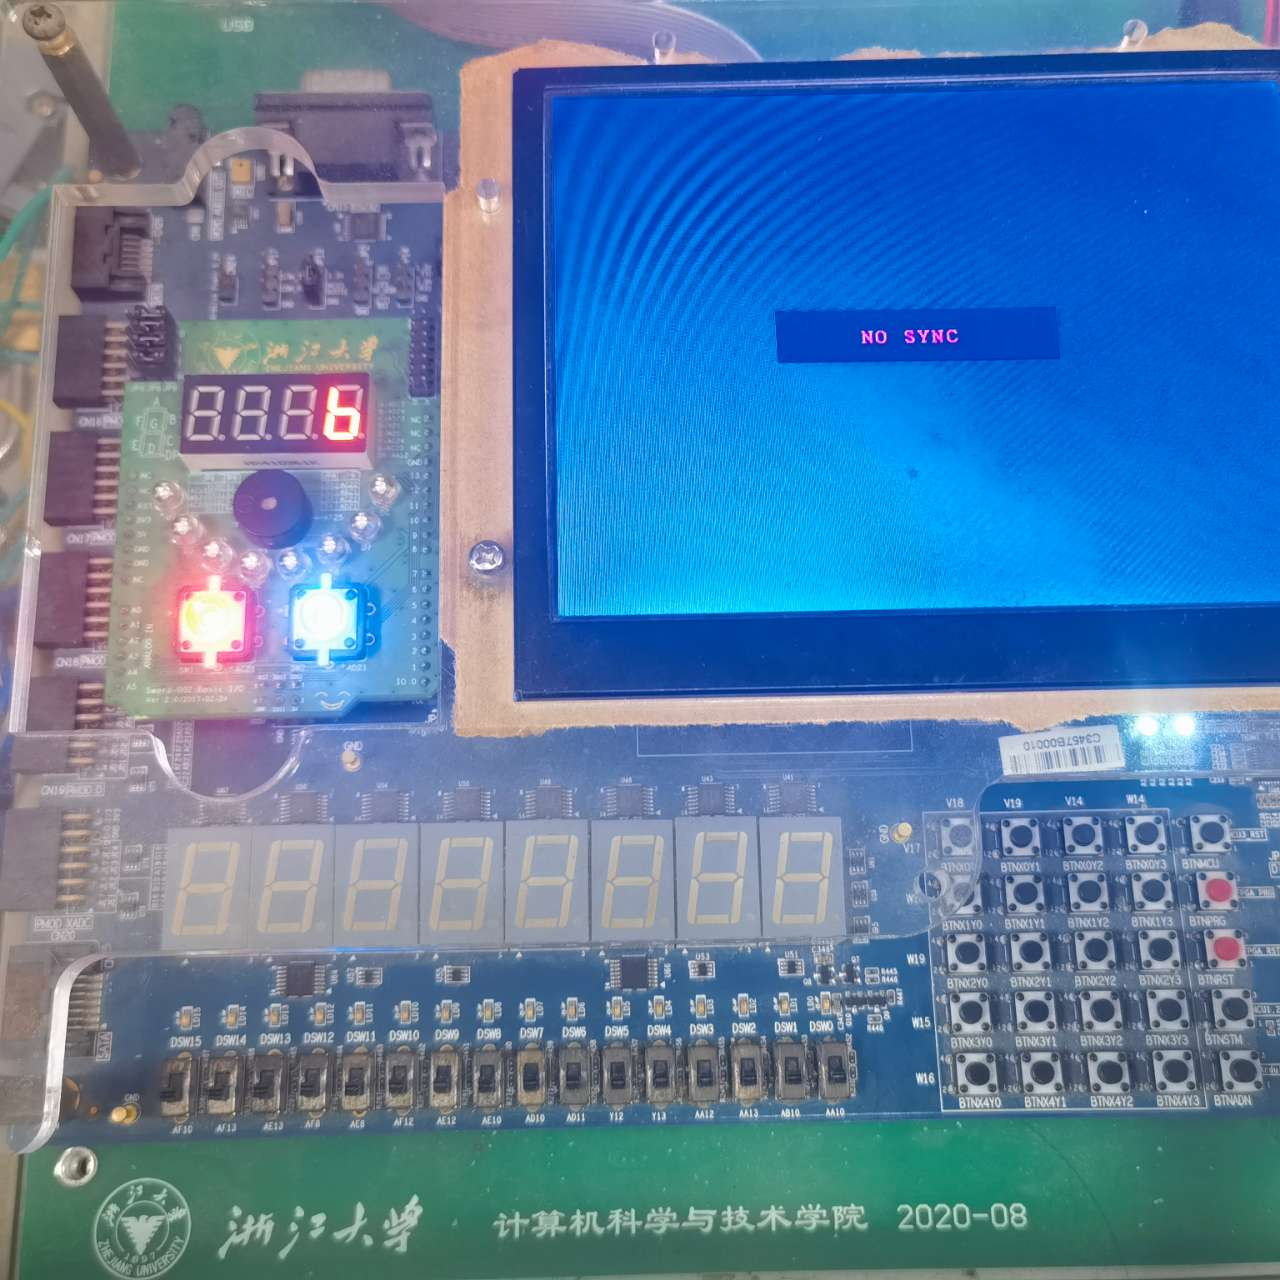
\includegraphics[width=0.5\textwidth]{lab10p/5.jpg}
    \caption{\label{Lab10}下板照片}
    \end{figure}

    \begin{figure}[H]
    \centering
    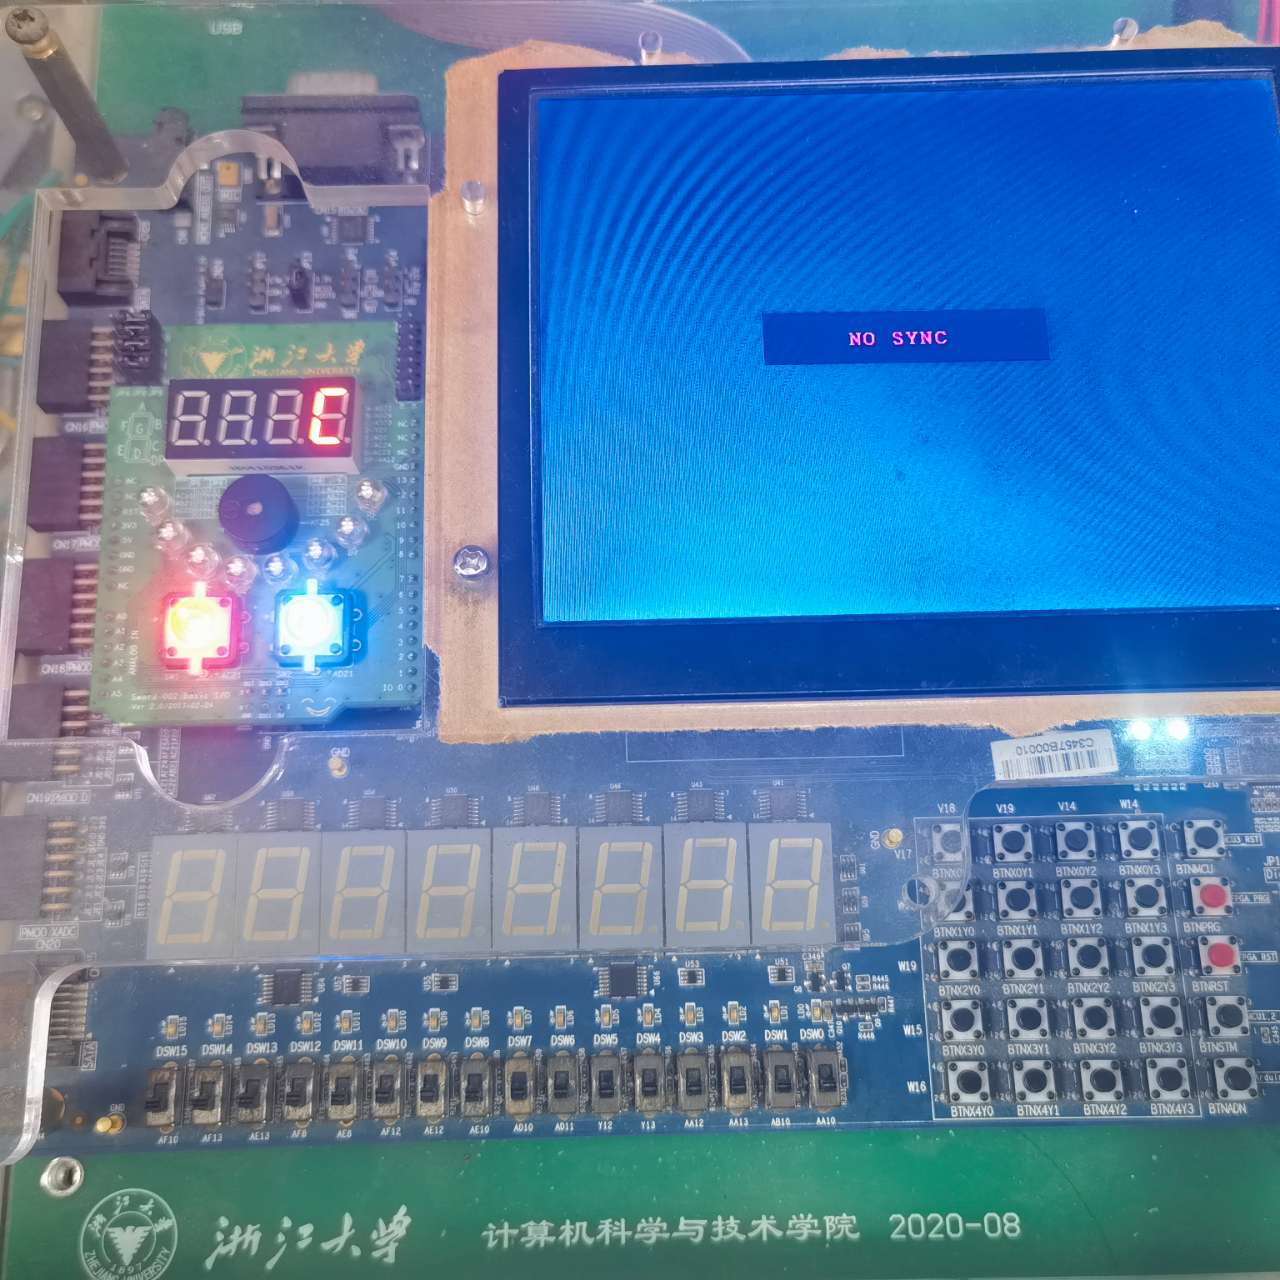
\includegraphics[width=0.5\textwidth]{lab10p/6.jpg}
    \caption{\label{Lab10}下板照片}
    \end{figure}
在下板成功后,可以看到数码管从0到F每次数字的变化间隔一秒,并且当计数器记录到F
时,此时Rc信号位1,输出的数字重置,下一时刻数码管显示的数字为1.

\subsubsection*{16位可逆二进制同步计数器:}
\begin{figure}[H]
    \centering
    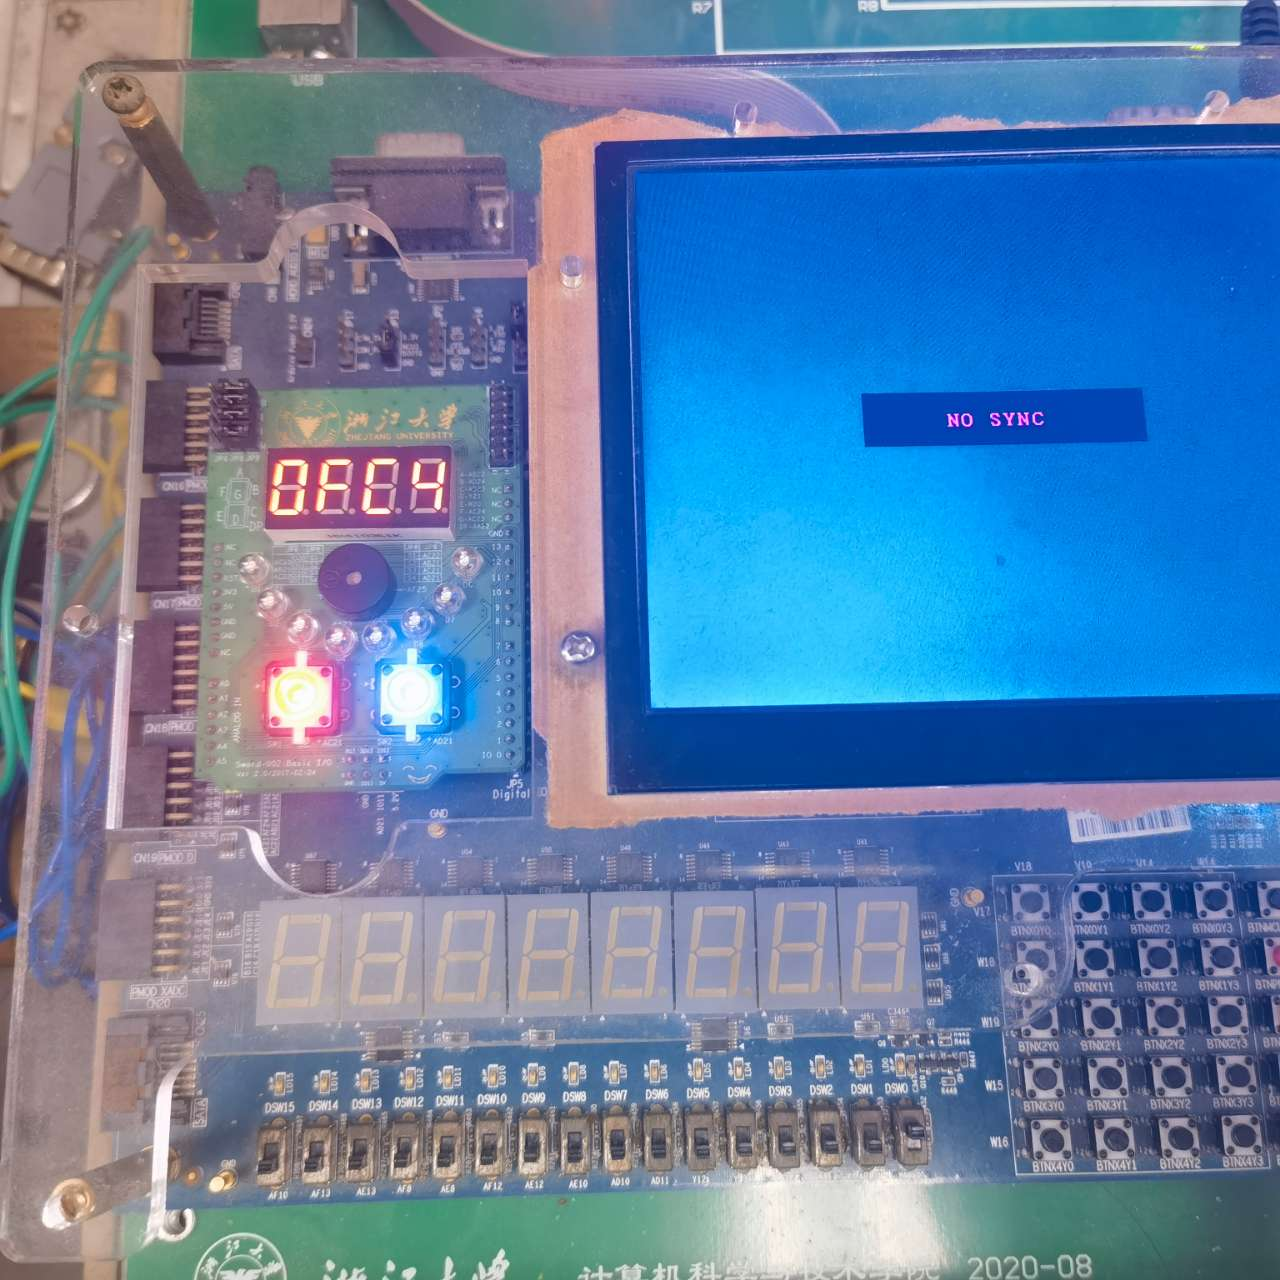
\includegraphics[width=0.5\textwidth]{lab10p/7.jpg}
    \caption{\label{Lab10}下板照片}
    \end{figure}

    \begin{figure}[H]
    \centering
    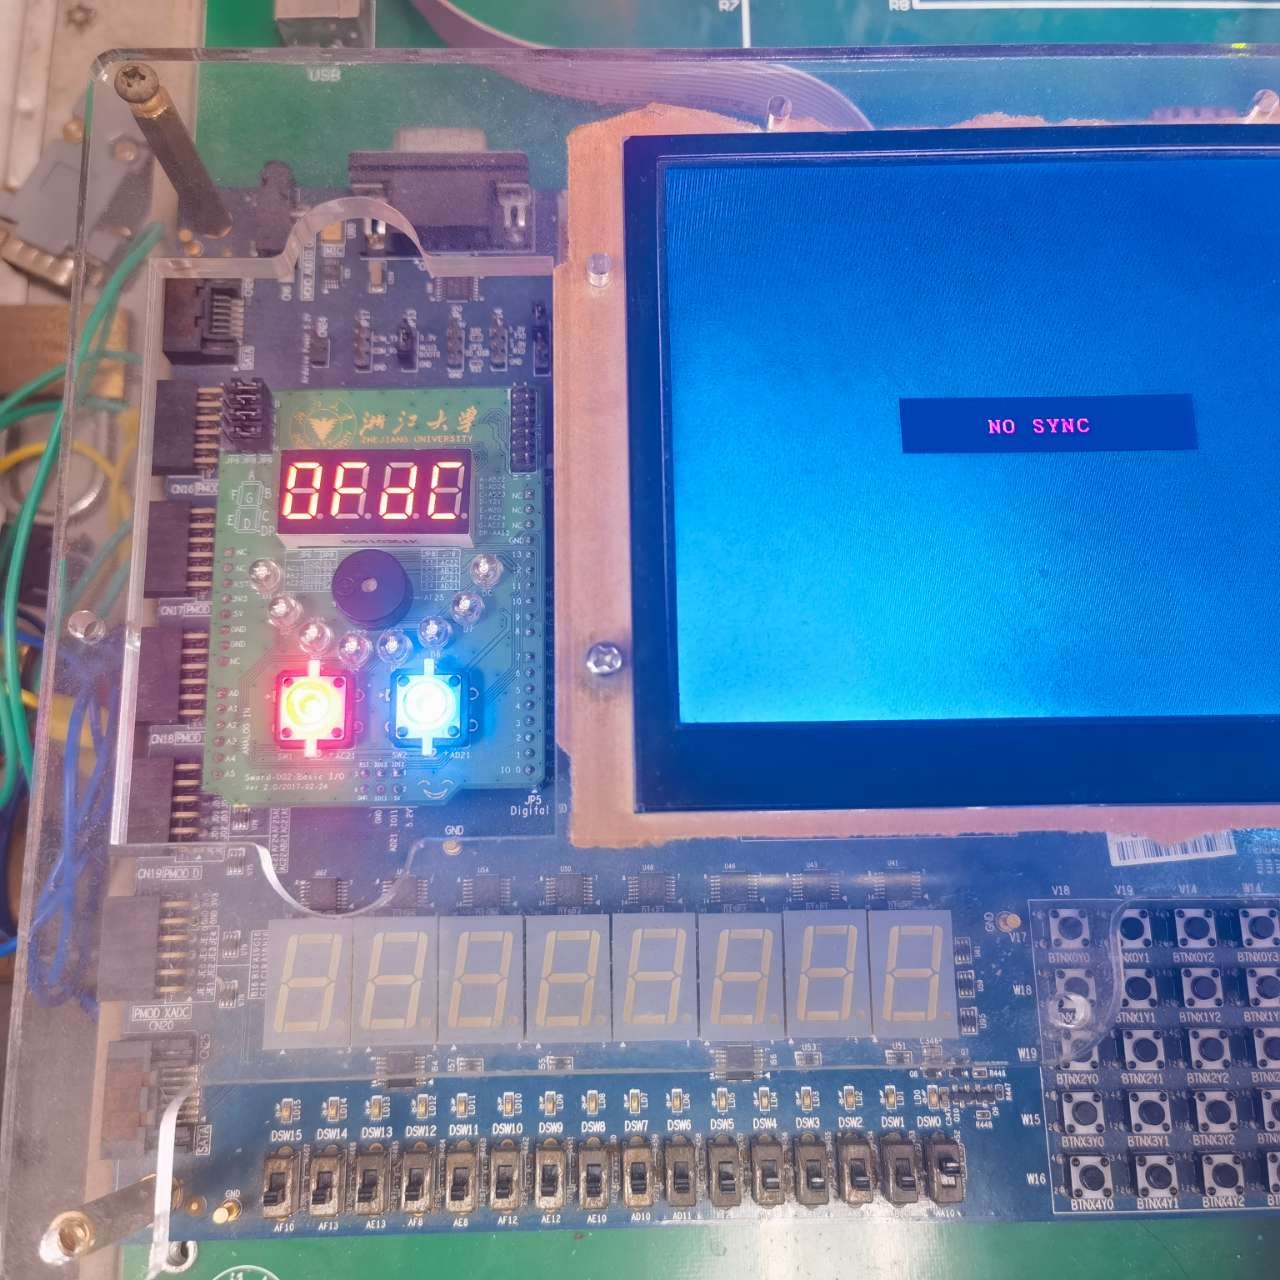
\includegraphics[width=0.5\textwidth]{lab10p/8.jpg}
    \caption{\label{Lab10}下板照片}
    \end{figure}
    
    \begin{figure}[H]
    \centering
    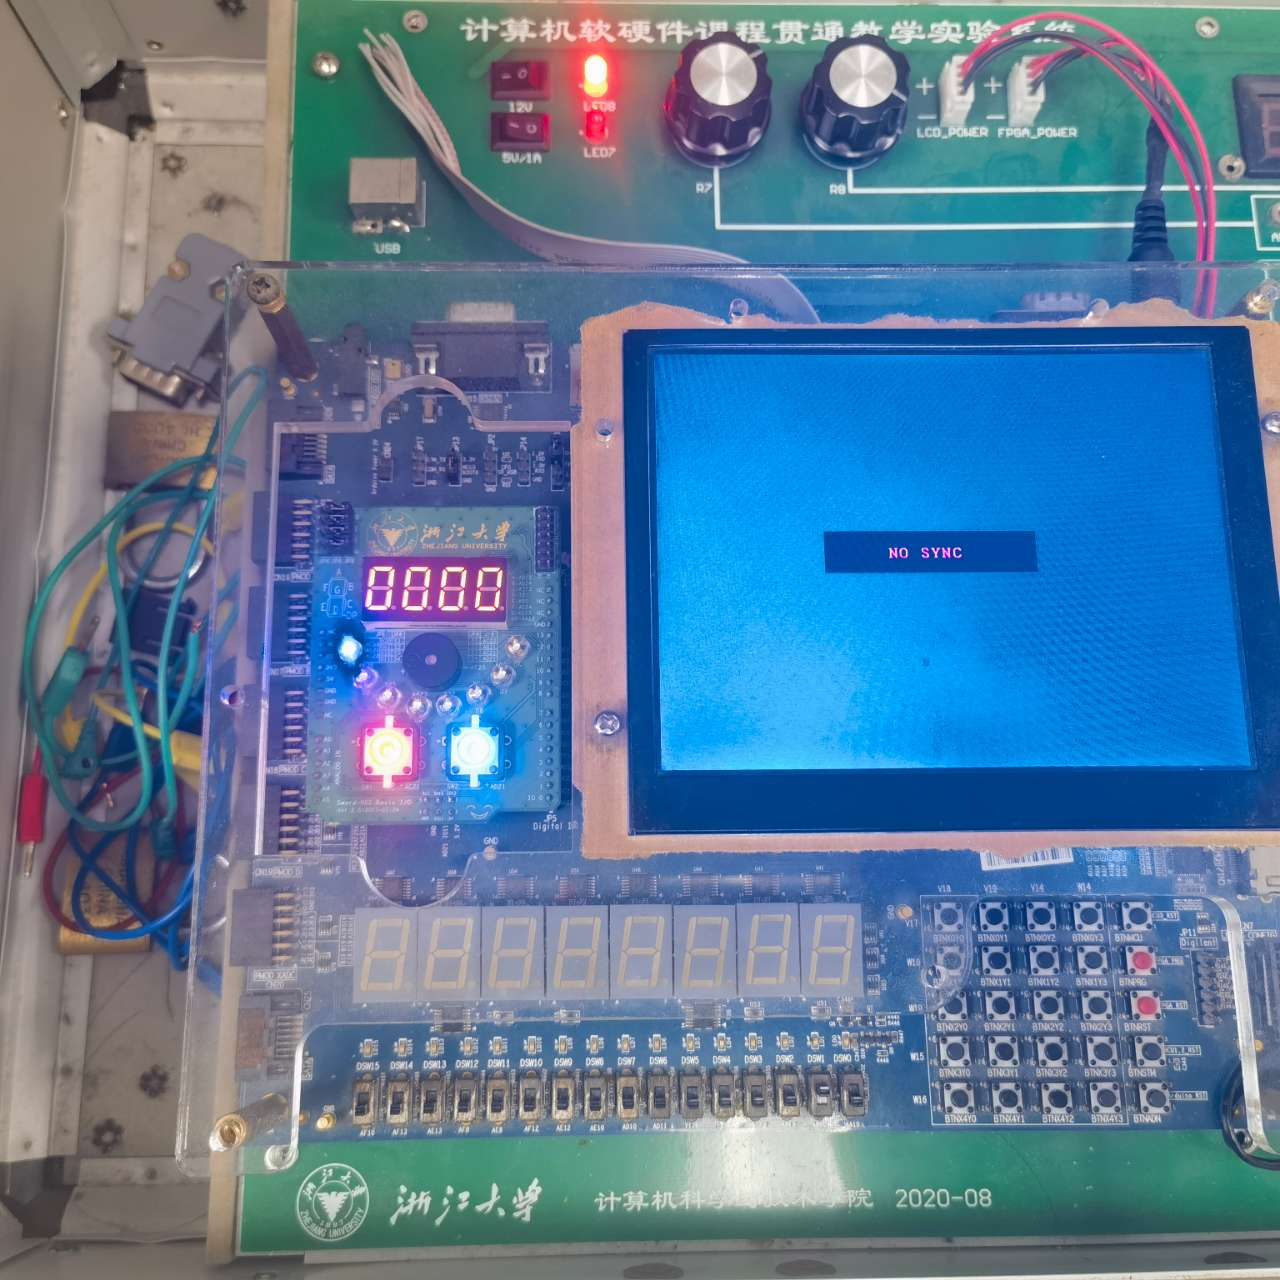
\includegraphics[width=0.5\textwidth]{lab10p/9.jpg}
    \caption{\label{Lab10}下板照片}
    \end{figure}

    \begin{figure}[H]
    \centering
    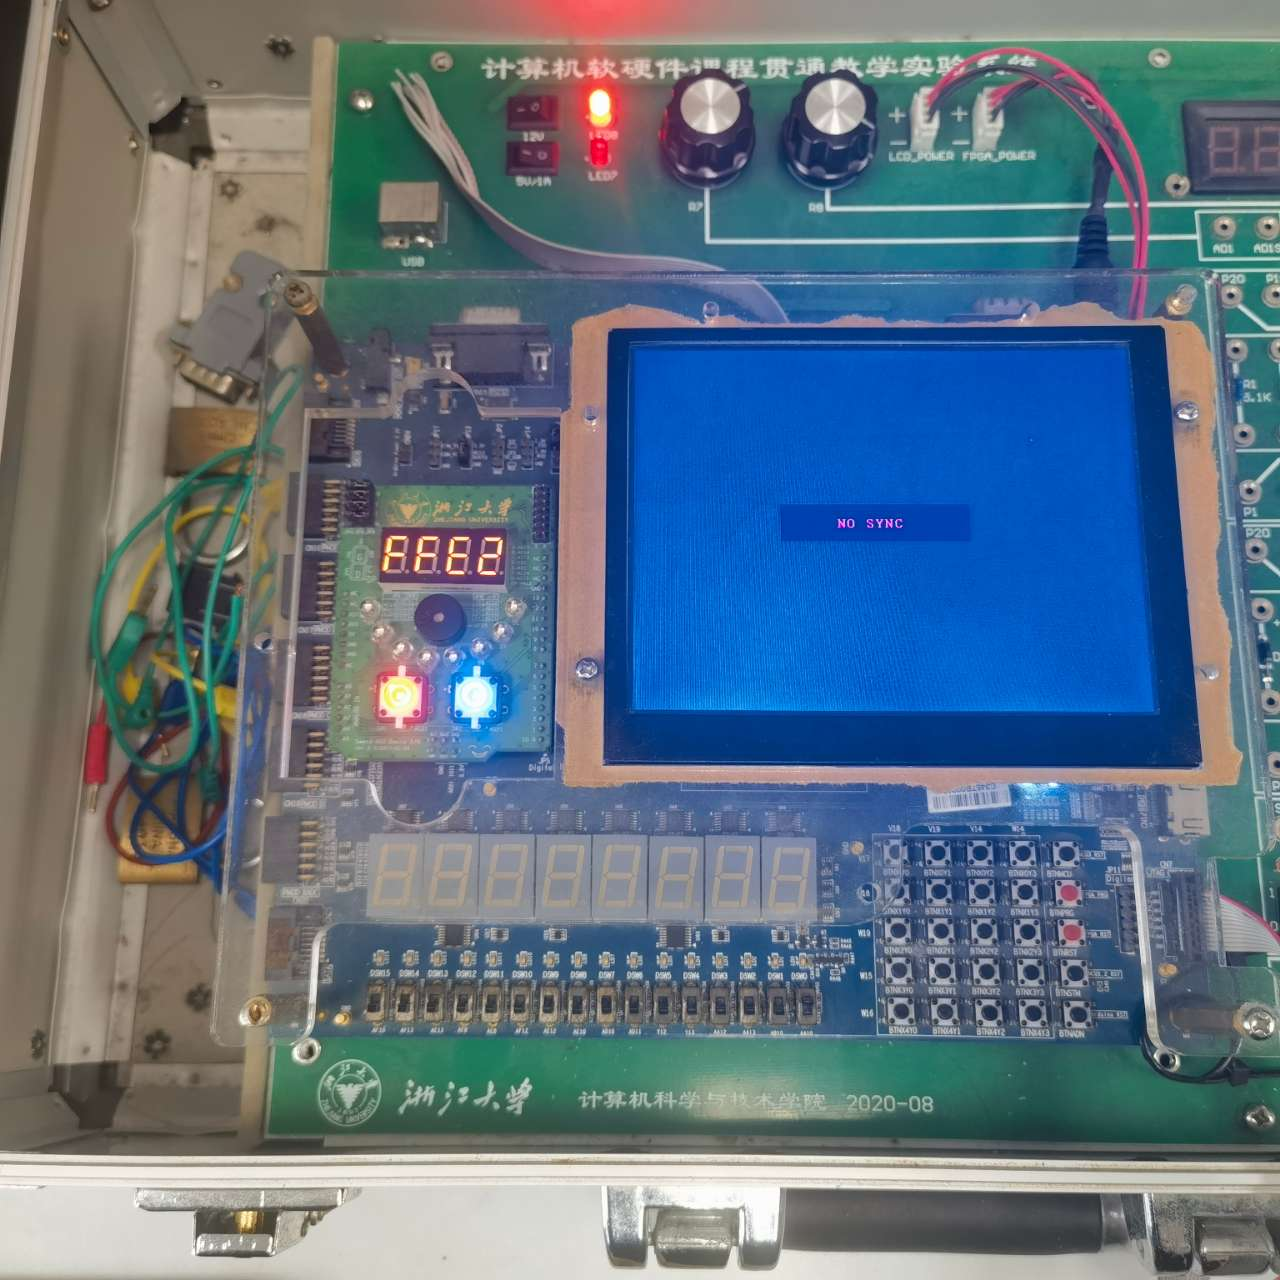
\includegraphics[width=0.5\textwidth]{lab10p/10.jpg}
    \caption{\label{Lab10}下板照片}
    \end{figure} 
    
    \begin{figure}[H]
    \centering
    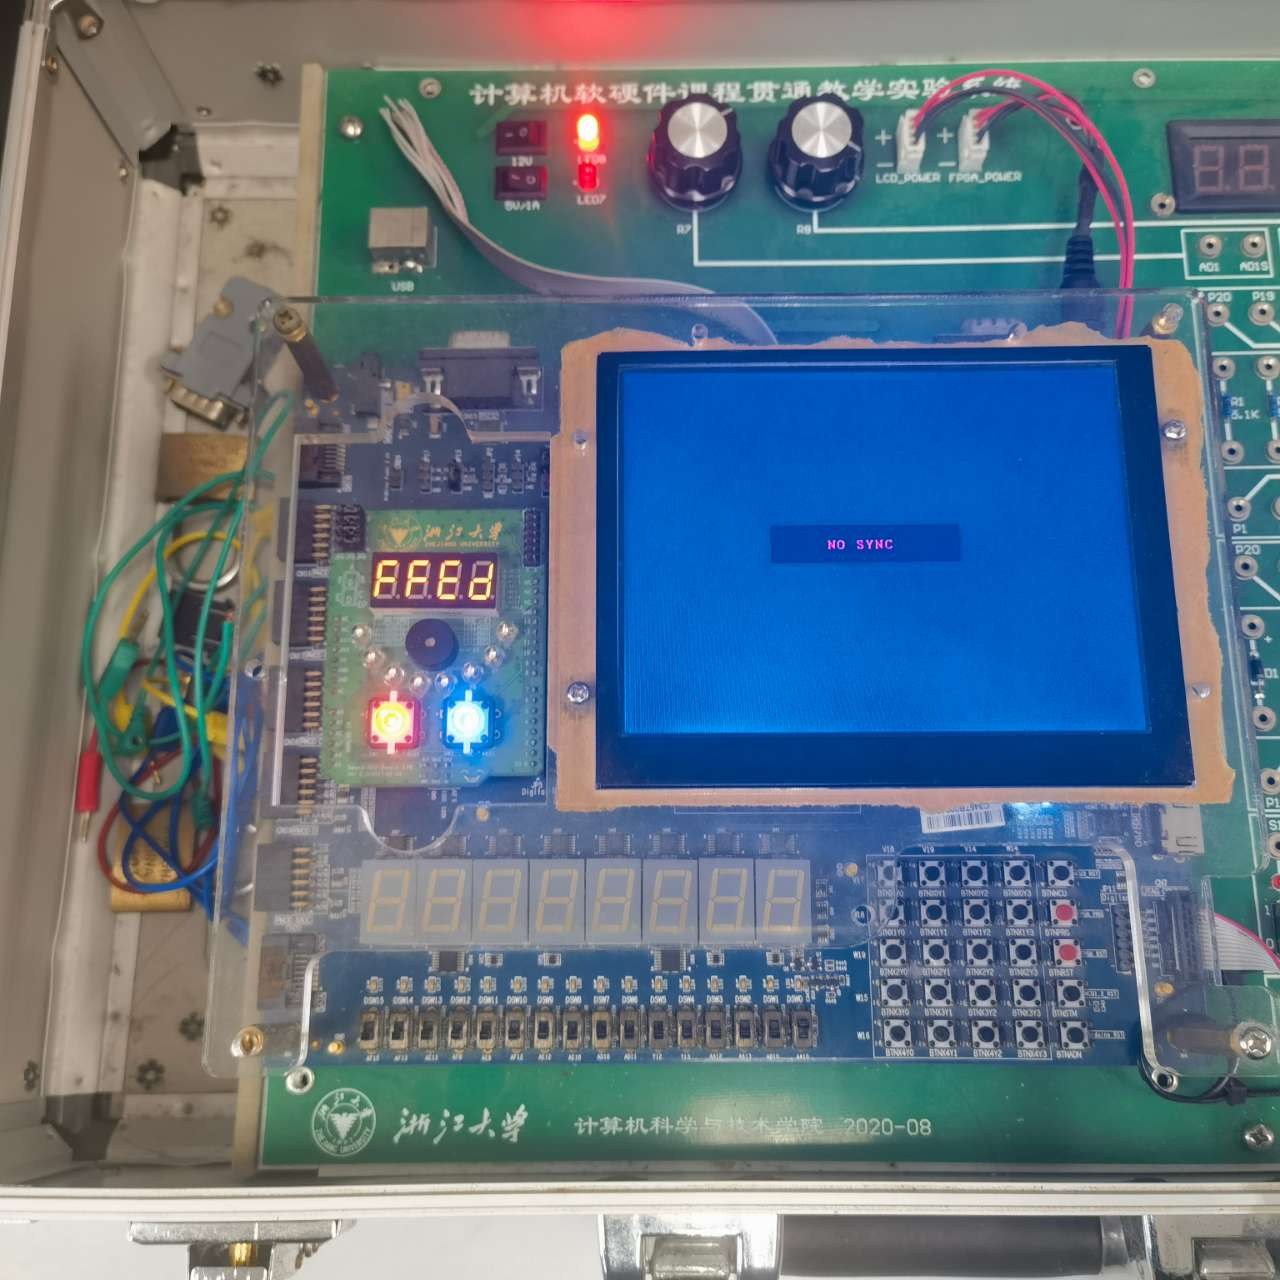
\includegraphics[width=0.5\textwidth]{lab10p/11.jpg}
    \caption{\label{Lab10}下板照片}
    \end{figure} 

    \begin{figure}[H]
    \centering
    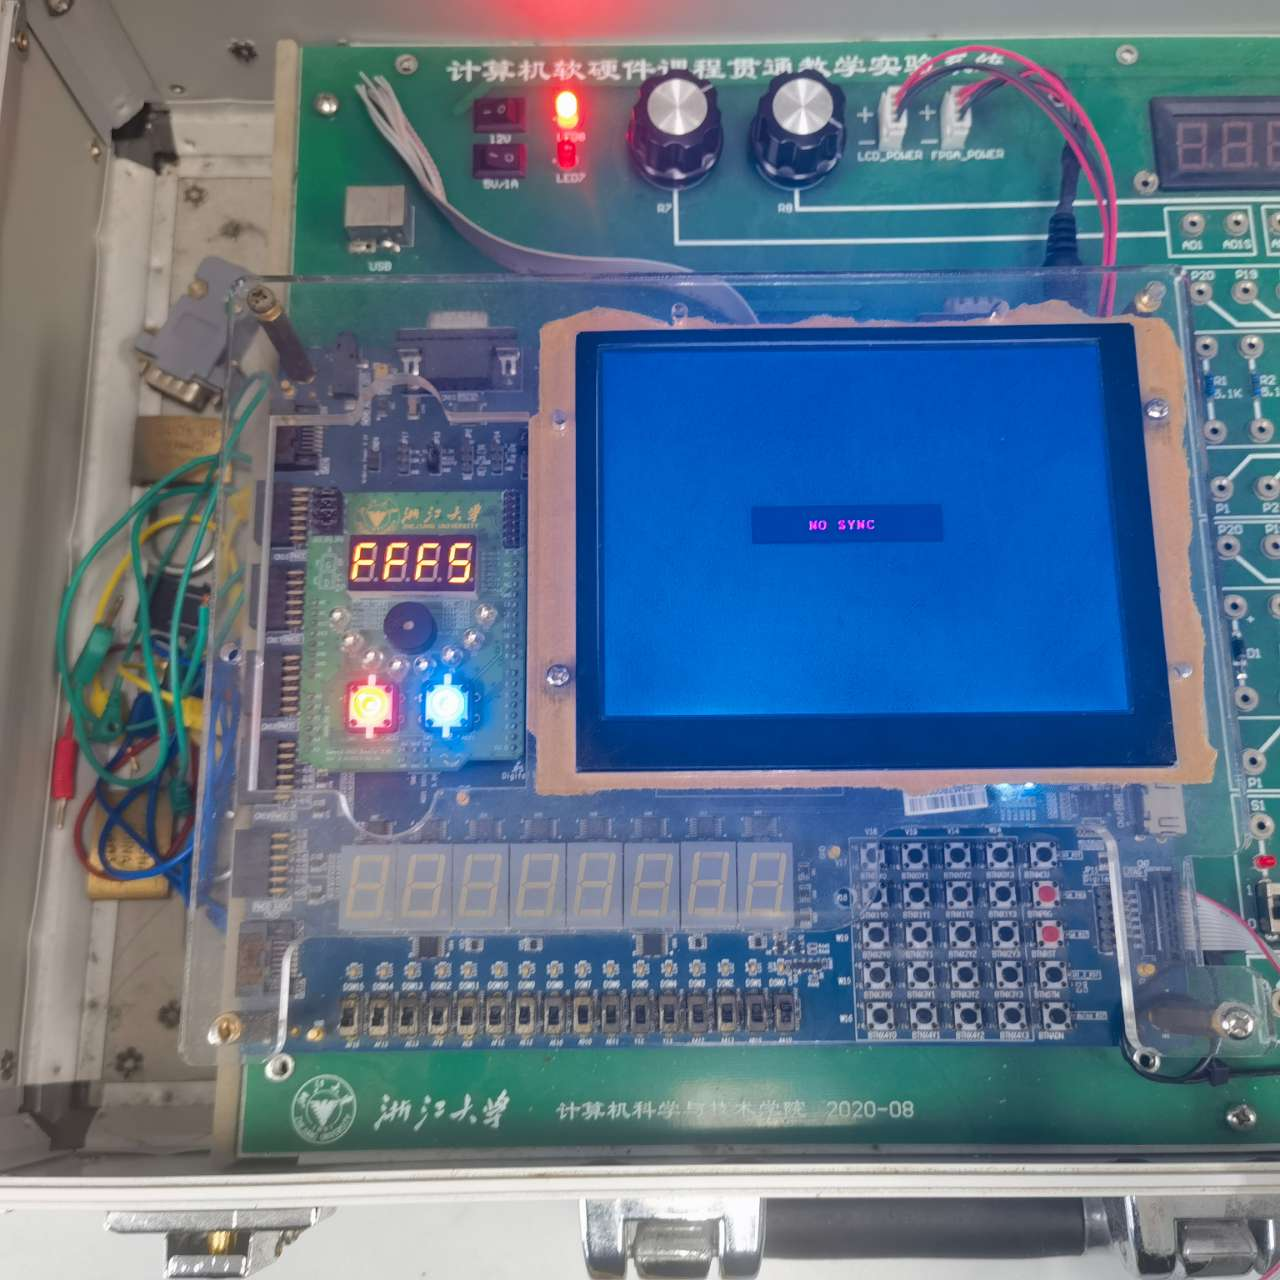
\includegraphics[width=0.5\textwidth]{lab10p/12.jpg}
    \caption{\label{Lab10}下板照片}
    \end{figure} 

    \begin{figure}[H]
    \centering
    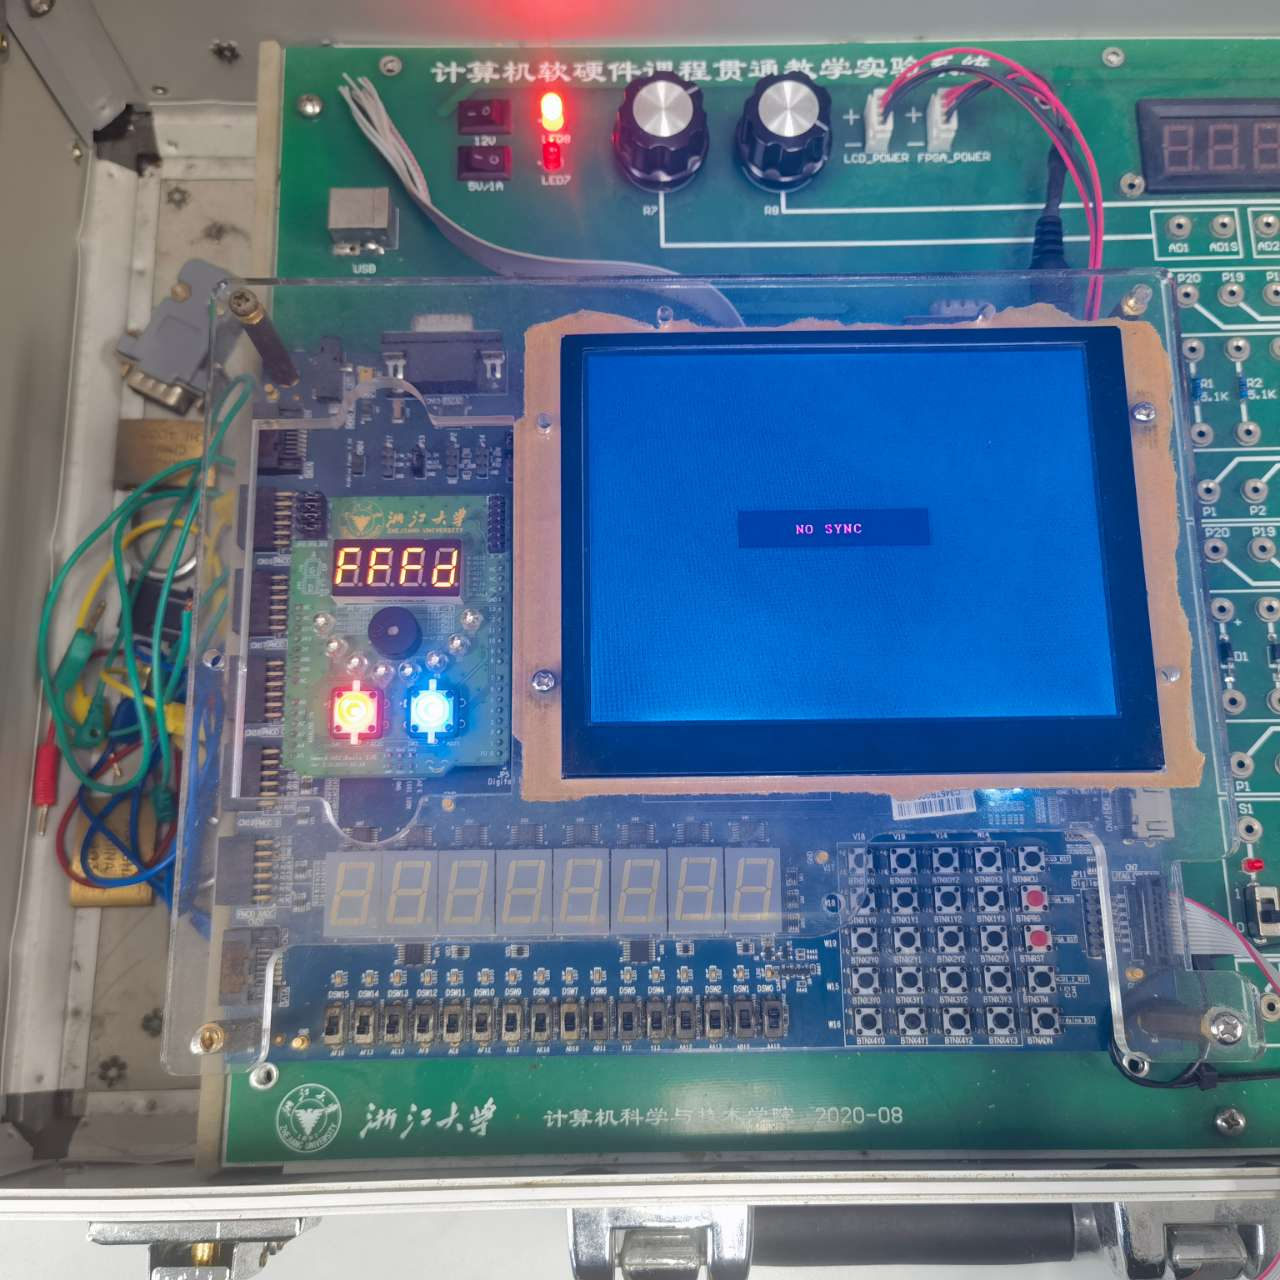
\includegraphics[width=0.5\textwidth]{lab10p/13.jpg}
    \caption{\label{Lab10}下板照片}
    \end{figure} 

当拨动s的对应开关时,s的信号值为1,此时进行正向计数的模式,每间隔0.1s数字
增加1,并且当数字增加到4'hFFFF时,Rc的信号灯闪亮,并且显示的数字从4'h0000
开始重新进行计数.

当闭合s的对应开关,s的信号值0,此时进行反向计数的模式,每间隔0.1s数字减少1,
并且当数字减少为4'h0000时,Rc的信号灯闪亮,并且显示的数字从4'hFFFF开始重新
依次递减计数.

同时在Bonus中设置了rst信号,当拨动对应的开关时数码管显示的数字归0,当关闭rst信号的
开关时,再重新开始计数.

\section*{三、讨论与心得}
在本次实验中遇到的主要问题是在本次实验中需要调用很多前面的实验使用的模块,
由于命名的不规范有一些对应的模块寻找起来比较困难,并且一些端口的命名的大小写和
写的top.v中有一些不同,一开始未加修改就直接进行了下一步的操作,产生了很多报错,
在修改端口名称之后问题就得以解决了.



\section*{四、Bonus}
在实验中完成了Bonus的要求.

\end{document}
